\documentclass[10pt,a4paper]{article}
\usepackage[utf8]{inputenc}
\usepackage{amsmath}
\usepackage{gensymb}
\usepackage{amsfonts}
\usepackage{siunitx}
\usepackage[european]{circuitikz}
\usepackage{geometry}
\newgeometry{tmargin=2cm, bmargin=2cm, lmargin=2cm, rmargin=2cm}
\usepackage{amssymb}
\usepackage{multirow}
\usepackage{polski}
\usepackage{graphicx}
\author{\textbf{T. Fąs}}
\title{\textbf{BADANIE WŁASNOŚCI FILTRÓW RC}}
\begin{document}
\maketitle

\begin{center}
\textbf{\subsection*{STRESZCZENIE}}
\end{center}
Celem doświadczenia było skonstruowanie filtru RC oraz zbadanie charakterystyki amplitudowej i fazowej jak i reakcji na różne, generowane sygnały. Zachowanie filtru było zgodne z oczekiwaniami i z przewidywaniami teoretycznymi.


\begin{center}
\textbf{\subsection*{WSTĘP}}
\end{center}

Filtry RC, składające się z opornika o oporze $R$ i kondensatora o oporze $C$ dzielą się na dwa rodzaje: filtry górno- i dolnoprzepustowe. Schematy obu tych filtrów przedstawiono na Rysunku 1.

\begin{figure}[h!]
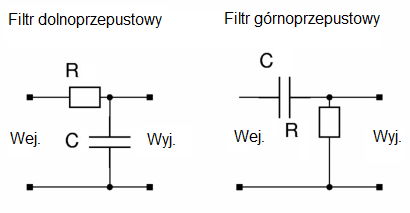
\includegraphics[width=10cm]{rap18rys11} 
\centering
\caption{Rodzaje filtrów RC.}
\end{figure}

W filtrach RC wyróżnia się częstość graniczną $\omega_{gr}=1/RC$, która stanowi umowną granicę między pasmem dobrego przenoszenia sygnału, a jego silnego tłumienia.
 W przypadku filtru dolnoprzepustowego sygnały o częstości znajdującej się poniżej częstości granicznej zostaną przepuszczane bez większych zmian, z kolei dla wyższych częstości sygnały zostaną wytłumione. Analogiczna sytuacja ma miejsce w przypadku filtru górnoprzepustowego; sygnały poniżej częstości granicznej są tłumione, a te powyżej są przepuszczane. Stosunek $T$ amplitudy napięcia wyjściowego $U_{wyj}$ do amplitudy napięcia wejściowego $U_{wej}$ dla filtru dolnoprzepustowego dane jest wzorem:
 
 \begin{equation}
 T=\dfrac{U_{wyj}}{U_{wej}}=\dfrac{1}{\sqrt{1+R^2C^2\omega^2}}
 \end{equation}
  Dodatkowo filtr dolnoprzepustowy jest, dla częstości powyżej częstości granicznej, również obwodem całkującym; napięcie na wyjściu jest proporcjonalne do całki napięcia na wejściu filtru. Z kolei filtr górnoprzepustowy różniczkuje napięcie wejściowe dla częstości poniżej częstości granicznej. 

W doświadczeniu badano wartość $T$ dla filtru dolnoprzepustowego w zależności od częstości sygnału wejściowego. Równolegle do pomiarów napięcia dokonywano też pomiarów przesunięcia fazowego $\phi$ sygnału wejściowego i wyjściowego. Zgodnie z przewidywaniami teoretycznymi, przesunięcia te powinny podlegać zależności:

\begin{equation}
\phi=\arctan{\left(\dfrac{1}{RC \omega}\right)}
\end{equation}

Zbadano również zakres częstości dla których obserwowano poprawne całkowanie sygnału. W tym celu sprawdzano wizualnie, obserwując wykresy sygnałów na oscyloskopie, czy sygnał wyjściowy jest poprawną całką sygnału wejściowego.

\begin{center}
\textbf{\subsection*{UKŁAD DOŚWIADCZALNY}}
\end{center}

Układ doświadczalny składał się z filtru dolnoprzepustowego, złożonego według schematu z Rysunku 1, oscyloskopu oraz generatora sygnałów. Generator został podłączony do filtru RC, a dalej do oscyloskopu. Dodatkowo bezpośrednio podłączono generator i oscyloskop, aby móc jednocześnie obserwować sygnał wejściowy i wyjściowy. Schemat układu przedstawiono na Rysunku 2.


\begin{figure}[h!]
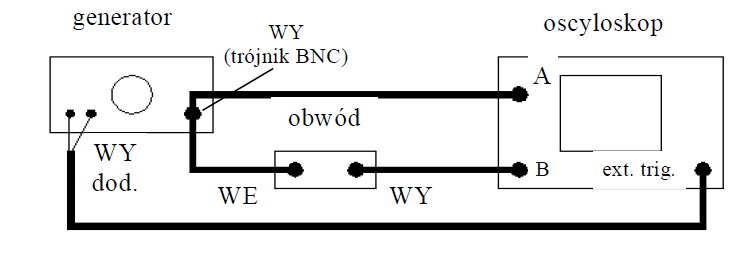
\includegraphics[width=10cm]{rap18rys112} 
\centering
\caption{Schemat układu \cite{r1}.}
\end{figure}

Po zakończeniu pomiarów zamieniono miejscami kondensator i opornik aby otrzymać filtr górnoprzepustowy. W trakcie dodatkowych pomiarów zbadano zakres poprawnego różniczkowania sygnału przez nowy obwód, jak i zmierzono jego częstość graniczną.

Wszystkie badane wartości były mierzone przy pomocy oscyloskopu, za wyjątkiem częstości prądu, która była odczytywano z generatora.

\begin{center}
\textbf{\subsection*{WYNIKI POMIARÓW}}
\end{center}
Wartości amplitudy napięcia wejściowego, wyjściowego, fazy i częstości są przedstawione w Tabeli 1.

\begin{table}[h!]
\centering
\caption{Wyniki pomiarów.}
\begin{tabular}{|c|c|c|c|c|c|c|c|}
\hline
$U_{wej}$ [V] & $U_{wyj}$ [mV] & $\omega/2\pi$ [s$^{-1}$] & $\phi$ [deg] & $U_{wej}$ [V] & $U_{wyj}$ [mV] & $\omega/2\pi$ [s$^{-1}$] & $\phi$ [deg] \\ \hline
5,04          & 4,28 V         & 1000                     & 32,4         & 4,8           & 0,0784         & 106000                   & 87,71        \\ \hline
4,8           & 0,756          & 10000                    & 79,92        & 4,8           & 0,0748         & 112000                   & 87,98        \\ \hline
4,8           & 0,482          & 16000                    & 82,5         & 4,8           & 0,0715         & 118000                   & 89,57        \\ \hline
4,8           & 0,358          & 22000                    & 84,47        & 4,8           & 0,067          & 124000                   & 89,11        \\ \hline
4,8           & 0,284          & 28000                    & 86,22        & 4,8           & 0,0674         & 130000                   & 89,36        \\ \hline
4,8           & 0,236          & 34000                    & 86,79        & 4,8           & 0,0625         & 136000                   & 88,04        \\ \hline
4,8           & 0,203          & 40000                    & 85,68        & 4,8           & 0,0601         & 142000                   & 89,49        \\ \hline
4,8           & 0,177          & 46000                    & 85,44        & 4,8           & 0,0579         & 148000                   & 89,47        \\ \hline
4,8           & 0,158          & 52000                    & 87,19        & 4,8           & 0,0556         & 154000                   & 89,44        \\ \hline
4,8           & 0,144          & 58000                    & 86,86        & 4,8           & 0,054          & 160000                   & 89,85        \\ \hline
4,8           & 0,131          & 64000                    & 87,12        & 4,8           & 0,0524         & 166000                   & 87,31        \\ \hline
4,8           & 0,12           & 70000                    & 87,23        & 4,8           & 0,0504         & 172000                   & 89,38        \\ \hline
4,8           & 0,112          & 76000                    & 88,09        & 4,8           & 0,0492         & 178000                   & 87,12        \\ \hline
4,8           & 0,104          & 82000                    & 87,04        & 4,8           & 0,0472         & 184000                   & 89,67        \\ \hline
4,8           & 0,094          & 88000                    & 89,84        & 4,8           & 0,046          & 190000                   & 88,12        \\ \hline
4,8           & 0,0876         & 94000                    & 87,97        & 4,8           & 0,0448         & 196000                   & 90,35        \\ \hline
4,8           & 0,0826         & 100000                   & 88,74        & 4,8           & 0,044          & 200000                   & 90,36        \\ \hline
\end{tabular}
\end{table}

Filtr dolnoprzepustowy dokonywał prawidłowego całkowania na przedziale od 6 kHz do 500 kHz.

 Dla przebudowanego filtra otrzymano przedział różniczkowania od 15 Hz do 400 Hz i odpowiadające im napięcia wyjściowe kolejno 40,0 mV oraz 830 mV dla napięć wejściowych kolejno 5,00 V i 5,08 V. Otrzymano również wartość $\omega_{gr}/2\pi=2,1$ kHz i wraz z $U_{wyj}=3,49$ V i $U_{wej}=4,92$ V. Podsumowanie tych danych przedstawiono w Tabeli 2.
 
 \begin{table}[h!]
\centering
\caption{Pomiary: przebudowany filtr.}
\begin{tabular}{|c|c|c|}
\hline
$U_{wej}$ [V] & $U_{wyj}$ [mV] & $\omega/2\pi$ [s$^{-1}$] \\ \hline
5,00          & 40,0           & 15                       \\ \hline
5,08          & 830            & 400                      \\ \hline
4,92          & 3,49 V        & 2100                     \\ \hline
\end{tabular}
\end{table}
 
 Dokonano również bezpośredniego pomiaru wartości oporu $R$ i pojemność $C$. Otrzymano wyniki $R=1004,35$ $\Omega$, $C=98,6$ nF. Stąd też wynika, iż wartość iloczynu RC wynosi 9,9$\cdot 10^{-5}$ s.
 
\begin{center}
\textbf{\subsection*{ANALIZA DANYCH}}
\end{center}

Dla danych z Tabeli 1 obliczono wartości $T$ oraz wykonano wykresy zależności $T(\omega)$ i $\phi(\omega)$. Do tych danych dopasowano zależności kolejno Równania 1 i Równania 2. 
Kierując się instrukcją oscyloskopu za niepewność napięcia przyjęto 2\% z kolei dla pomiarów fazy przyjęto 3$^\circ$ ze względu na wahania tej wartości w trakcie pomiaru.

 Dane wraz z krzywymi najlepszego dopasowania przedstawiono na Rysunku 3 i Rysunku 4.



\begin{figure}[h!]
\includegraphics[width=12cm]{rap18rys1} 
\centering
\caption{Dopasowanie: transmitancja $T$.}
\end{figure}


\begin{figure}[h!]
\includegraphics[width=12cm]{rap18rys2} 
\centering
\caption{Dopasowanie: faza $\phi$.}
\end{figure}



 Dla Rysunku 3 otrzymano wartość parametru $RC=(9,127\pm0,058)\cdot ^{-5}$ s i wartość $\chi^2=53,80$, a dla Rysunku 4 $RC=(9,40 \pm 0,39)\cdot 10^{-5}$ s, $\chi^2=5,29$. W obu przypadkach wartość krytyczna $\chi^2_{kryt}=47,40$. Jak widać krzywa dopasowania dla zależności $T(\omega)$ nie przechodzi testu $\chi^2$ pomimo doskonałego dopasowania wizualnego, z kolei dopasowanie dla $\phi(\omega)$ przechodzi test bez problemu. 
 
 Dla dalszej analizy oba wykresy przedstawiono w skali logarytmicznej, kolejno na Rysunku 5 i Rysunku 6. 
 



\begin{figure}[h!]
\includegraphics[width=12cm]{rap18rys5} 
\centering
\caption{Logarytm: transmitancja $T$.}
\end{figure}


\begin{figure}[h!]
\includegraphics[width=12cm]{rap18rys6} 
\centering
\caption{Logarytm: faza $\phi$.}
\end{figure}




Ujawniają się tu niedoskonałość dopasowania krzywej $T(\omega)$. Jednakże wizualne dopasowanie oraz wartość $\chi^2$, która jest bliska wartości krytycznej pozwala założyć, iż wykres ten jest zgodny z przewidywaniami teoretycznymi.


Otrzymane wartości parametru $RC$ są ze sobą zgodne na mocy testu $3\sigma$, a średnia ważona obu wielkości wynosi $(9,1326\pm0,057)\cdot10^{-5}$ s. Wartość ta nie jest jednak zgodna z wartością parametru $RC$ obliczoną z bezpośrednich pomiarów oporu i pojemności. Wziąwszy jednak pod uwagę fakt, iż różnica między tymi wielkościami wynosi zaledwie 
7,7$\cdot 10^{-6}$ s, to można uznać obie wartości za akceptowalnie zgodne ze sobą.

Wartość $\omega_{gr}/2\pi$ dla wyznaczonej średniej ważonej wynosi 1741 Hz, a dla bezpośredniego pomiaru wynosi 1607 Hz. 

W przypadku przebudowanego filtra oszacowano wartość częstości granicznej na 2100 Hz, dla której $T=0,709$. Jak widać wartość ta jest wyższa od wartości granicznych dla filtru całkującego, choć powinna być identyczna. Być może przebudowanie filtra w jakiś sposób zmieniło jego parametry (większa ilość cyny mogła zwiększyć opór i pojemność), choć nie wydaję się to być głównym powodem rozbieżności wyników.

Aby zbadać granice poprawnego całkowania sygnału generowano na wejściu sygnał prostokątny i obserwowano, w jakim przedziale ten sygnał najlepiej przekształca się w sygnał trójkątny. Otrzymano przedział od 6 kHz do 500 kHz. Poniżej tego przedziału wpuszczany sygnał za bardzo przypominał eksponens, a powyżej szumy oraz efekt Gibbsa za bardzo zniekształcały obraz. 

Badając filtr różniczkujący generowano sygnał trójkątny i otrzymywano sygnał prostokątny w przedziale od 15 Hz do 400 Hz. W tym przypadku szumy i efekt Gibbsa bardzo szybko zniekształcały obraz.

W obu przypadkach otrzymano przedziały zgodne z oczekiwaniami: dla układu całkującego częstości są znacznie większe od częstości granicznej, a dla układu różniczkującego znacznie od niej niższe. Tak więc można uznać działanie obu tych układów za zgodne z teorią.

\begin{center}
\textbf{\subsection*{DYSKUSJA WYNIKÓW I WNIOSKI}}
\end{center} 

Pomimo drobnej rozbieżności wyników układ RC zachowywał się zgodnie z przewidywaniami teoretycznymi: wytłumiał sygnały po przekroczeniu częstości granicznej, całkował i różniczkował w przedziałach, w których następowało silne tłumienie, a obliczone wartości częstości granicznych były ze sobą zgodne. Tak więc można uznać uzyskane wyniki za satysfakcjonujące, a układ za zgodny z teorią.

\begin{center}
\begin{thebibliography}{9}

 \bibitem{r1}
 Praca zbiorowa,
 \emph{Instrukcja do ćwiczenia "Obwody prądu zmiennego:
Badanie własności filtrów RC"},
 FUW, Warszawa, 2016, s. 2.

 
 \end{thebibliography}

\end{center}


\end{document}